\documentclass[12pt, a4paper]{article}

\usepackage{amsmath, amssymb, amsthm}  % for math symbols
\usepackage[margin=1in]{geometry}      % for formatting the margins
\usepackage{graphicx, float}           % for including images
\graphicspath{{plots/}}                % for image path
\usepackage{caption}                   % for image captions
\usepackage{multicol}                  % for multiple columns
\usepackage{enumitem}                  % more enumerate functions
\usepackage{xcolor}                    % for coloured text
\usepackage{natbib}                    % for bibliography
\usepackage{libertine}                 % for fonts
\usepackage{booktabs}
\usepackage{hyperref}
\hypersetup{
	colorlinks = true,
	linkcolor = blue,
	urlcolor  = blue,
	citecolor = black,
	anchorcolor = blue}
\urlstyle{same}
\usepackage{microtype}


% Additional Formatting Changes
\setlength{\parindent}{0pt}
\setlength{\parskip}{6pt}
\setlist[itemize]{topsep=0pt}
\setlist[enumerate]{topsep=0pt}
\setlength{\bibsep}{0pt}

%
% ===== DOCUMENT STARTS HERE =======
% you do not have to modify anything above
% if you do not wish to (but you indeed can)
%
\begin{document}
	
\title{Simulation-Based Inference for an Adaptive-Network Epidemic Model}
\date{11 April 2026}
\maketitle

{\bf Group Composition:}
\begin{enumerate}
    \item Lou Jia Jun, A0299872A, e1354238@u.nus.edu
\end{enumerate}

{\bf Github Repository:} \url{https://github.com/SharkWhale9/ST3247-Assignment/}

\section{Introduction}
The classical SIR (Susceptible–Infected–Recovered) model is one of the most widely used frameworks for studying the spread of infectious diseases. In most of these network models, the epidemic propagates on a fixed network. In reality, however, individuals adapt their behaviour in response to the epidemic: susceptible individuals may avoid infected contacts, leading to a dynamically evolving network. This project studies a stochastic SIR epidemic model on such an adaptive network, introduced by \citet{gross2006epidemic}.

\subsection{The Model}
We consider a population of $N = 200$ agents interacting on an undirected Erdos-Renyi random graph $G(N,p)$ with $p=0.05$. This graph serves as the contact network and yields an expected degree $\approx 10$. Each node is in one of three states: susceptible (S), infected (I), or recovered (R). The simulation runs for $T=200$ discrete time steps. At each discrete time step, three synchronous processes occur:
\begin{enumerate}
    \item Infection: Each susceptible node connected to an infected neighbour becomes infected with probability $\beta$.
    \item Recovery: Each infected node (including those newly infected in the current step) recovers with probability $\gamma$.
    \item Rewiring: For each S–I edge, the susceptible node breaks the connection with probability $\rho$ and reconnects to a uniformly chosen non-neighbor. Note that this new connection could be with an infected agent.
\end{enumerate}
The three unknown parameters and their priors are summarised in Table 1.

\begin{table}[h]
\centering
\begin{tabular}{lll}
\hline
\textbf{Parameter} & \textbf{Meaning}  & \textbf{Prior} \\ \hline
$\beta$   & Infection probability per S–I edge per time step      & $\text{Uniform}(0.05, 0.50)$ \\ \hline
$\gamma$  & Recovery probability per infected agent per time step & $\text{Uniform}(0.02, 0.20)$ \\ \hline
$\rho$    & Rewiring probability per S–I edge per time step       & $\text{Uniform}(0.0, 0.8)$   \\ \hline
\end{tabular}
\caption{Model parameters \& prior distributions}
\end{table}

\subsection{Objective}
The goal of this project is to infer the unknown parameter vector $\theta = (\beta, \gamma, \rho)$ from observed data of 40 independent realisations generated by this model. 

For each realisation, we observe:
\begin{itemize}
    \item the infected fraction time series
    \item the rewiring count time series
    \item the final degree distribution
\end{itemize}
Importantly, the underlying contact network and individual-level state transitions are never observed.

\subsection{Why the Likelihood Is Intractable}
The rewiring mechanism couples the disease dynamics to the network topology, creating a feedback loop: the spread of infection reshapes the contact structure, which in turn changes how the disease spreads \citep{gross2006epidemic}. Evaluating the exact likelihood $p(\text{data} \mid \theta)$ would require marginalising over every possible joint sequence of infection events, recoveries, and network rewirings. Because both agent states and network evolve stochastically, the number of such trajectories grows exponentially with $N$ and $T$, making exact computation infeasible. 

We therefore turn to simulation-based inference methods that do not require explicit likelihood evaluation for inference about the model parameters. We begin with Approximate Bayesian Computation as a tractable baseline.

\section{Summary Statistics Design}
Summary statistics are used in ABC to reduce high-dimensional data into a low-dimensional set of features that are sensitive to parameters of interest. Effective statistics allow the partial posterior to closely match the true full posterior. The six statistics used throughout this project are described in Table 2, together with the parameter each targets and its theoretical motivation. The validity of these summary statistics is discussed in Section 3.4.

\begin{table}[H]
\centering
\small
\begin{tabular}{p{2.75cm}p{3.25cm}p{1.5cm}p{7cm}}
\toprule
\textbf{Statistic} & \textbf{Description} & \textbf{Target} & \textbf{Theoretical Justification} \\
\midrule

peak
& Maximum infected proportion
& $\beta$, $\gamma$
& The epidemic peak occurs when the number of susceptible individuals drops to $S = \gamma / \beta$ making it sensitive to both \citep{Kermack1927}.\\
\addlinespace

peak\_t
& Time of maximum infection prop.
& $\beta$
& The early exponential growth rate $r \approx \beta - \gamma$ determines how quickly infections rise. Increasing $\beta$ accelerates growth and shifts the peak earlier \citep{Kermack1927}. \\
\addlinespace

auc
& Area under infection curve
& $\gamma$
& The area under the infection curve reflects total infectious burden. Longer infectious periods (smaller $\gamma$) increase cumulative infections \citep{Kermack1927}. \\
\addlinespace

peak\_rew
& Maximum single step rewiring count
& $\rho$, $\beta$
& Rewiring can only occur along SI edges, so peak rewiring activity reflects both the rewiring rate and how many SI edges transmission has created \citep{gross2006epidemic}. \\
\addlinespace

rew\_per\_infected
& Total rewiring per unit of cumulative infection
& $\rho$, $\beta$, $\gamma$
& Rewiring causes infected nodes to lose contacts at rate $\rho$, reducing their effective degree and increasing the epidemic threshold \citep{gross2006epidemic}. Normalising total rewiring by cumulative infections reflects this contact-loss mechanism while controlling for overall epidemic size.\\
\addlinespace

var\_deg
& Variance of final degree distribution
& $\rho$
& As susceptible nodes repeatedly rewire connections, the degree distribution is altered, with greater rewiring increasing the spread \citep{shaw2008fluctuating}. \\

\bottomrule
\end{tabular}
\caption{Chosen summary statistics \& description}
\end{table}

\section{Basic Rejection ABC}
\subsection{Algorithm}
The rejection ABC algorithm proceeds as follows: For $i = 1, \dots, N_\text{sim}$
\begin{enumerate}
    \item Draw from prior: $\theta_i \sim \pi(\theta)$ 
    \item Simulate data: $y_i \sim f(\cdot \mid \theta_i)$ 
    \item Compute summary statistics: $s_i = S(y_i)$
    \item Compute distance: $d_i = \|s_i - s_\text{obs}\| $
    \item Accept $\theta_i$ only if $d_i \leq \varepsilon$
\end{enumerate}

For this implementation, we used the unweighted Euclidean distance to compute $d_i$ due to its simplicity. To ensure comparability across summaries with different scales, each summary statistic was normalised using the empirical mean and standard deviation of all simulated summaries: 
$$ S^{\text{norm}} = \frac{S - \bar{S}}{\hat{\sigma}}$$
We used $N_\text{sim} = 10^6$ simulations and set $\varepsilon$ to the 1st percentile of the empirical distance distribution. The choice of this threshold reflects the bias-variance trade-off: larger $\varepsilon$ reduces Monte Carlo variance due to a larger sample size but increases approximation bias. Given the large number of simulations performed, the 1\% threshold provides a reasonable trade-off between accuracy and computational efficiency \citep{beaumont2002approximate}.

\subsection{Approximate Posterior Distribution}
\begin{table}[h]
\centering
\begin{tabular}{lcccc}
\toprule
Param          & mean   & std    & 95\% CI              & contraction \\ \midrule
$\hat{\beta}$  & 0.1770 & 0.0382 & {(}0.1123, 0.2578{)} & 67.7\%      \\
$\hat{\gamma}$ & 0.0881 & 0.0160 & {(}0.0613, 0.1214{)} & 66.4\%      \\
$\hat{\rho}$   & 0.3051 & 0.0624 & {(}0.1940, 0.4299{)} & 70.5\%      \\ \bottomrule
\end{tabular}
\caption{ABC Posterior estimates}
\end{table}

\begin{figure}[h!]
    \centering
    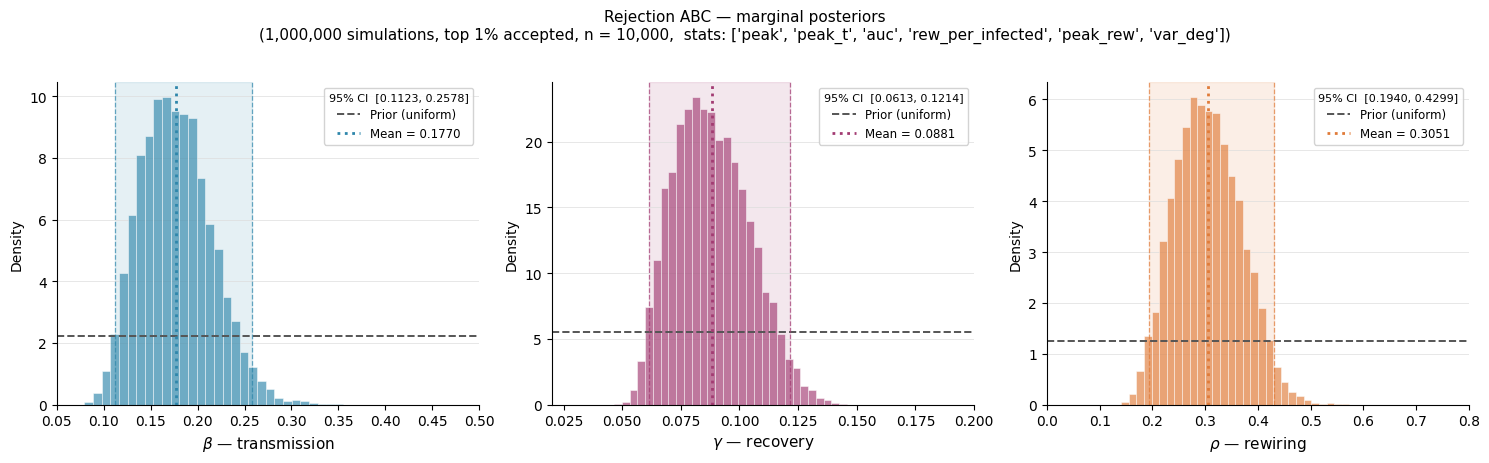
\includegraphics[width=\textwidth]{post_dist.png}
    \caption{Approximate posterior distribution (ABC)}
    \label{fig:post_dist}
    \centering
\end{figure}

Contraction measures the relative reduction in 95\% credible interval width relative to the prior. A value above ~50\% is generally considered informative. The substantial contraction across all three parameters indicates that the observed data are informative and that the ABC procedure is not merely reproducing the prior.

\begin{figure}[h!]
    \centering
    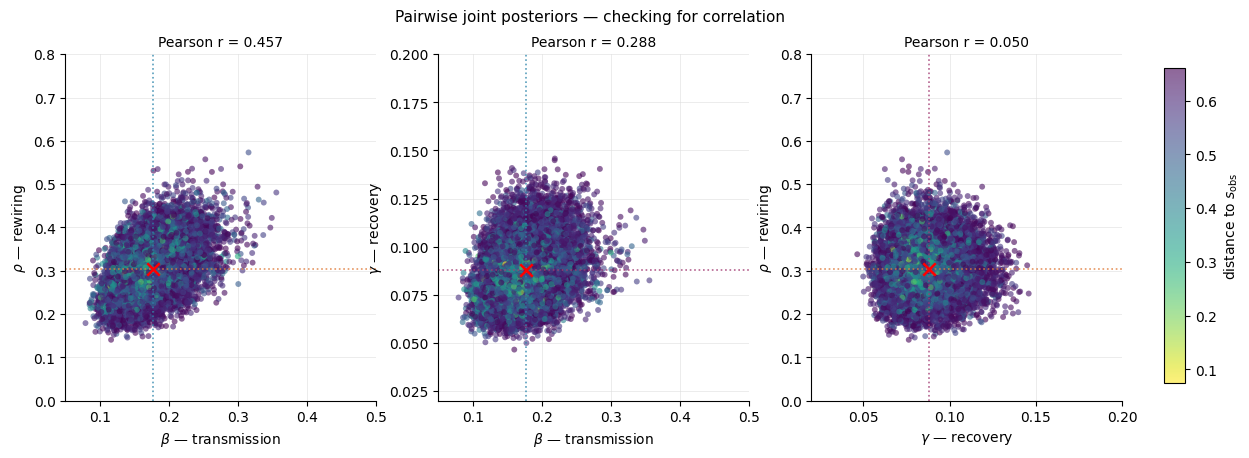
\includegraphics[width=\textwidth]{joint_post.png}
    \caption{Joint posterior distribution (ABC)}
    \label{fig:joint_post}
    \centering
\end{figure}

The pairwise joint posterior (Figure 2) reveals a moderate positive correlation between $\beta$ and $\rho$ ($r = 0.452$). This is structurally expected as $\beta$ and $\rho$ can both suppress the epidemic through different mechanisms: higher $\beta$ increases transmission while higher $\rho$ removes S–I edges through rewiring, resulting in the two parameters partially compensating for each other in producing similar epidemic trajectories. The correlation between $\beta$ and $\gamma$ is weaker ($r = 0.297$), indicating that the chosen summaries were effective at discriminating between transmission and recovery.

\subsection{Assessment of Posterior Quality}
 \begin{figure}[h]
    \centering
    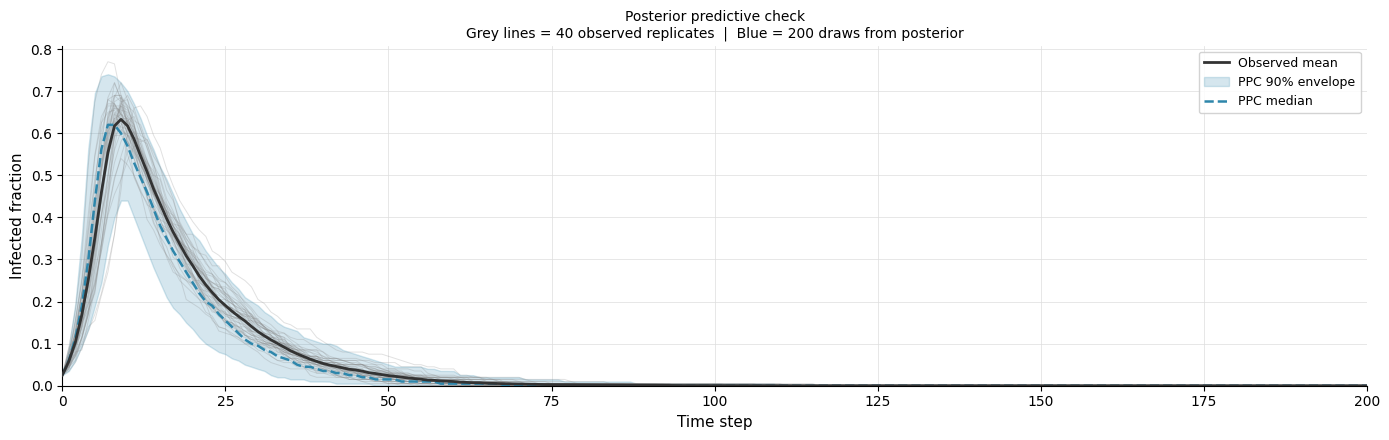
\includegraphics[width=\textwidth]{visual_ppc.png}
    \caption{Visual posterior predictive check}
    \label{fig: VPPC}
    \centering
\end{figure}

Figure 3 shows the visual posterior predictive check. For each of 200 draws from the accepted posterior, the simulator was run once to produce a replicated epidemic trajectory. The resulting 95\% predictive envelope and median trajectory are overlaid against the 40 observed replicates and their mean. The observed mean closely tracks the PPC median throughout the epidemic, and the 95\% envelope contains the majority of observed trajectories in all time steps.

\begin{figure}[h]
    \centering
    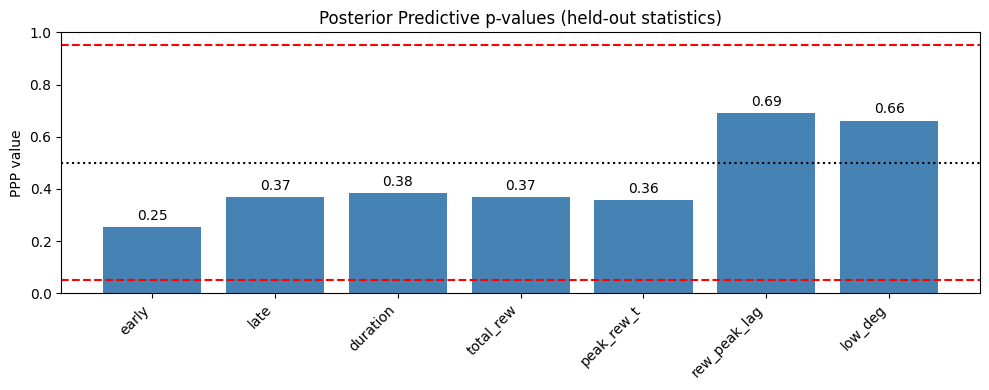
\includegraphics[width=\textwidth]{PPC.png}
    \caption{Posterior predictive p-values}
    \label{fig: PPC}
    \centering
\end{figure}

To quantify model adequacy beyond visual inspection, we adopt the posterior predictive checking framework of \citet{Gelman1996}. For each accepted posterior sample ($\beta_i,\gamma_i,\rho_i$), we replicate a trajectory $y^\text{rep}$ and compute a set of test statistics $T(y^\text{rep})$. To avoid circular validation, the statistic should not be one that was used for fitting. We then compare these replicated statistics to the observed values. The posterior predictive p-value is defined as
$$PPP = P(T(y^\text{rep}) \geq T(y^\text{obs}) \mid y^\text{obs})$$
and estimated as the fraction of replicates where $T(y^\text{rep}) \geq T(y^\text{obs})$. 

Unlike classical p-values, PPP values are conservative and tend to concentrate around 0.5, so only extreme values $(< 0.05 \text{ or} > 0.95)$ indicate model misfit. All held-out statistics yield PPP values within this range (Figure 4), confirming that the fitted model provides an adequate generative description of the data.


\subsection{Quality of Summary Statistics} 
\subsubsection{Validity of Theoretical Justifications}
To validate the theoretical choices in Section 2, Table 4 reports the empirical Pearson correlation between each summary statistic and each parameter across all $N_\text{sim}$ simulations. 

\begin{table}[H]
\centering
\begin{tabular}{|l|c|c|c|}
\hline
                   & $\beta$   & $\gamma$  & $\rho$    \\ \hline
peak               & 0.609614  & -0.531830 & -0.314908 \\ \hline
peak\_t            & -0.426697 & -0.102336 & 0.014125  \\ \hline
auc                & 0.158341  & -0.770066 & -0.120015 \\ \hline
peak\_rew          & 0.409111  & -0.247365 & 0.683368  \\ \hline
rew\_per\_infected & -0.366914 & 0.480650  & 0.620875  \\ \hline
var\_deg           & -0.320179 & 0.035452  & 0.652972  \\ \hline
total\_rew         & -0.049743 & -0.148137 & 0.612046  \\ \hline
\end{tabular}
\caption{Correlation between summary statistics \& model parameters}
\end{table}

These empirical correlations (Table 4) confirm the theoretical justification provided in Section 2. Epidemic-shape summaries (peak, peak\_t, auc) are primarily informative about $\beta$ and $\gamma$, while network summaries (peak\_rew, rew\_per\_infected, var\_deg) are primarily informative about $\rho$. Notably, total\_rew is weakly correlated with both $\beta$ and $\gamma$ ($|r| < 0.15$), whereas rew\_per\_infected shows stronger discrimination across all three parameters. Substituting total\_rew for rew\_per\_infected increased the $\beta$-$\rho$ correlation from 0.457 to 0.667, and the $\gamma$-$\rho$ correlation from 0.050 to 0.260, confirming that normalising by cumulative infections better decouples $\rho$ from the other parameters.

\subsubsection{Comparison with classical SIR model}
To demonstrate the necessity of network summaries for this model class, we repeated the ABC procedure using only the trajectory-based statistics commonly used in classical SIR models: \{peak, peak\_t, auc, early, duration\}, where early is the early growth rate of infection. 

\begin{figure}[h!]
    \centering
    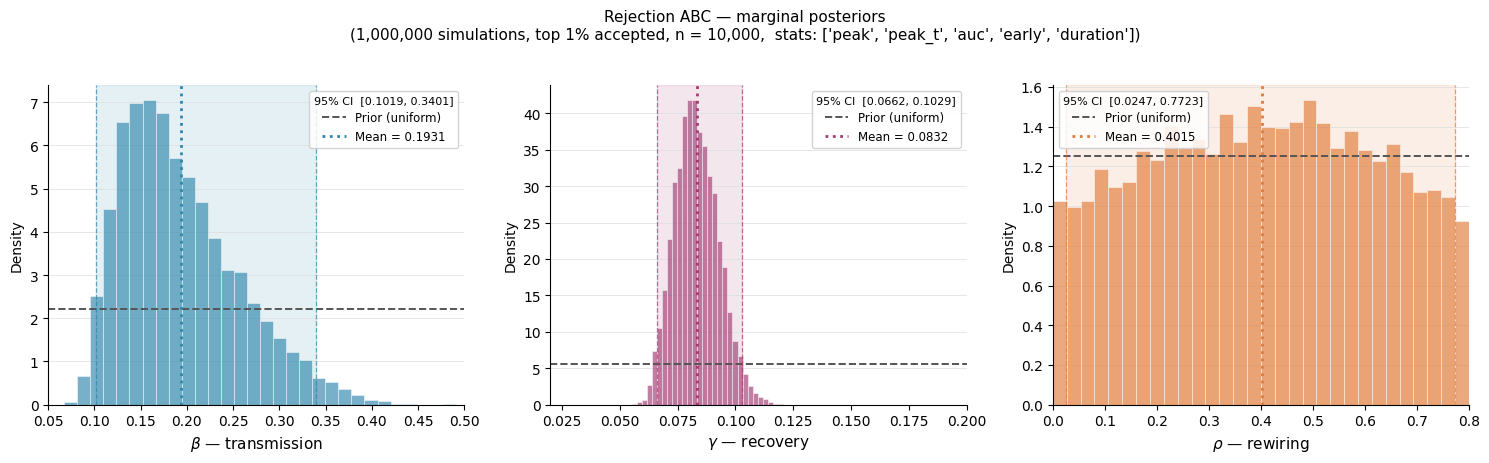
\includegraphics[width=\textwidth]{post_dist_classic.png}
    \caption{Approximate posterior distribution (classical summary statistics)}
    \label{fig:post_dist_classic}
    \centering
\end{figure}

\begin{figure}[h!]
    \centering
    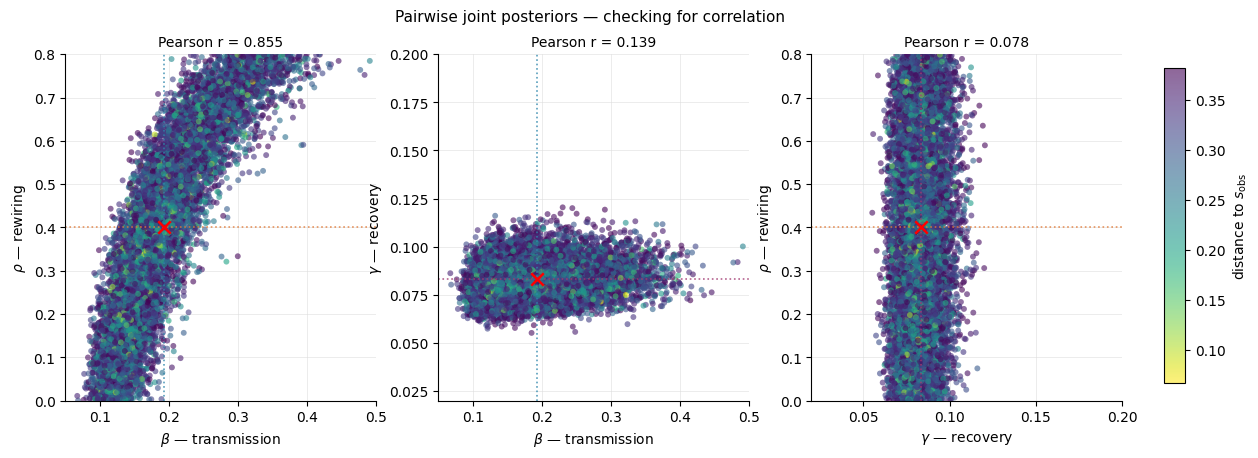
\includegraphics[width=\textwidth]{joint_post_classic.png}
    \caption{Joint posterior distribution (classical summary statistics)}
    \label{fig:joint_post_classic}
    \centering
\end{figure}

Under this specification, the posterior for $\rho$ exhibits minimal contraction (6.6\%) and the posterior correlation between $\beta$ and $\rho$ increases to 0.855, indicating strong confounding between transmission and rewiring effects. This suggests that classical SIR-inspired summaries do not contain sufficient information to separately identify these mechanisms in the adaptive-network setting.

\section{Advanced Methods}
\subsection{Limitations of Rejection ABC}
While rejection ABC provides a simple framework for simulation-based inference, it suffers from several practical limitations. First, it is computationally inefficient as the majority of simulated parameter proposals are discarded. Second, the method depends critically on the choice of $\varepsilon$, which is typically chosen heuristically and has no direct likelihood-based interpretation. These limitations motivate more efficient and better-grounded alternatives, such as regression-adjusted ABC and Bayesian Synthetic Likelihood.

\subsection{Bayesian Synthetic Likelihood}
The concept of synthetic likelihood was originally proposed by \citet{wood_statistical_2010}, while \citet{Price02012018} were the first to consider in detail its use for Bayesian inference. 
Bayesian Synthetic Likelihood (BSL) assumes that the summary statistics follow an approximate multivariate Gaussian distribution conditional on the parameters:
$$ S \mid \theta \sim \mathcal{N}(\mu(\theta), \Sigma(\theta))$$
The mean and covariance are estimated via repeated simulations at each proposed $\theta$. This yields an approximate likelihood that can be used in a standard Metropolis-Hastings MCMC framework, avoiding the need for a tolerance parameter altogether.

\subsubsection{Algorithm}
\begin{enumerate}
\item \textbf{Simulation:} For a proposed parameter vector $\theta^* = (\beta^*, \gamma^*, \rho^*)$, generate $M$ independent datasets from the epidemic simulator and compute their corresponding summary statistics $\{S(y^{(i)})\}_{i=1}^M$.

\item \textbf{Moment estimation:} Estimate the conditional mean and covariance of the summaries:
$$
\hat{\mu}(\theta^*) = \frac{1}{M} \sum_{i=1}^M S(y^{(i)}), 
\quad
\hat{\Sigma}(\theta^*) = \text{Cov}\left(S(y^{(1)}), \dots, S(y^{(M)})\right).
$$

\item \textbf{Synthetic likelihood:} Approximate the likelihood of the observed summaries $S_{\text{obs}}$ using a multivariate Gaussian:
$$
\hat{p}(S_{\text{obs}} \mid \theta^*) = \mathcal{N}(S_{\text{obs}}; \hat{\mu}(\theta^*), \hat{\Sigma}(\theta^*)).
$$

\item \textbf{MCMC update:} Embed the synthetic likelihood in a Metropolis--Hastings scheme:
$$
\pi(\theta^* \mid S_{\text{obs}}) \propto \pi(\theta^*) \, \hat{p}(S_{\text{obs}} \mid \theta^*),
$$
and accept or reject proposals using the standard MH acceptance ratio.
\end{enumerate}

\subsubsection{Posterior Distribution and Interpretation}
\begin{table}[H]
\centering
\begin{tabular}{lcccc}
\toprule
Param          & mean   & std    & 95\% CI              & contraction \\ \midrule
$\hat{\beta}$  & 0.1567 & 0.0212 & {(}0.1190, 0.2011{)} & 81.7\%      \\
$\hat{\gamma}$ & 0.0807 & 0.0053 & {(}0.0703, 0.0913{)} & 88.3\%      \\
$\hat{\rho}$   & 0.3062 & 0.0284 & {(}0.2563, 0.3695{)} & 85.9\%      \\ 
\bottomrule
\end{tabular}
\caption{Posterior estimates and credible interval contraction for model parameters (BSL)}
\end{table}
    
Under BSL, all three parameters exhibit stronger posterior contraction than under rejection ABC, with narrower credible intervals and reduced marginal variance (Table 5), reflecting more efficient use of the joint information in the summaries.

\begin{figure}[h!]
        \centering
        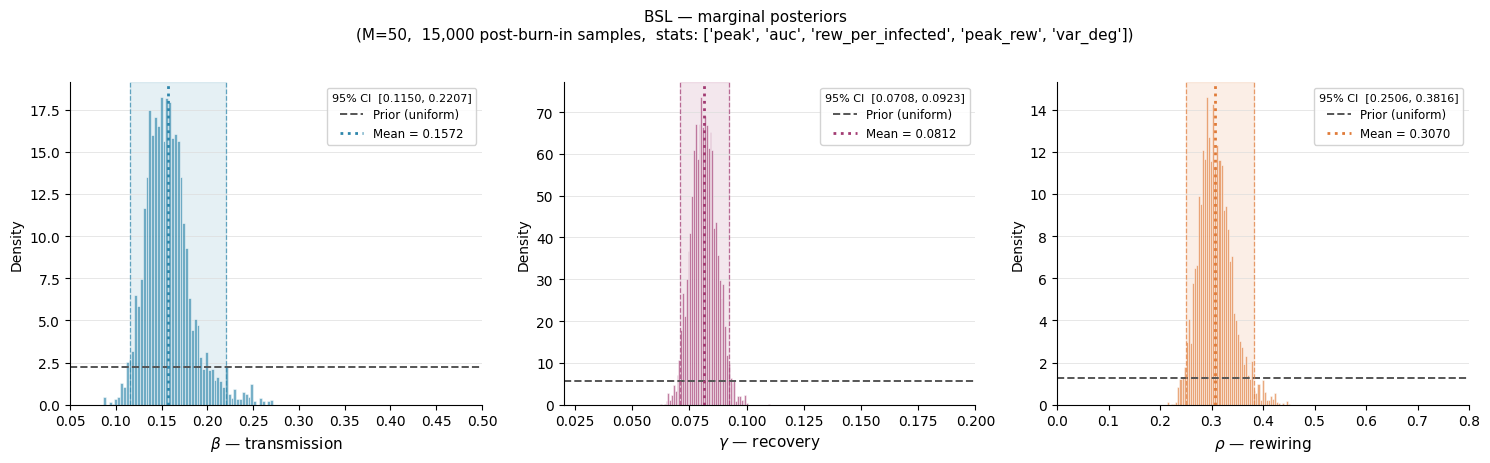
\includegraphics[width=\textwidth]{post_dist_bsl.png}
        \caption{Approximate posterior distribution (BSL)}
        \label{fig:post_dist_BSL}
        \centering
    \end{figure}

    \begin{figure}[h!]
        \centering
        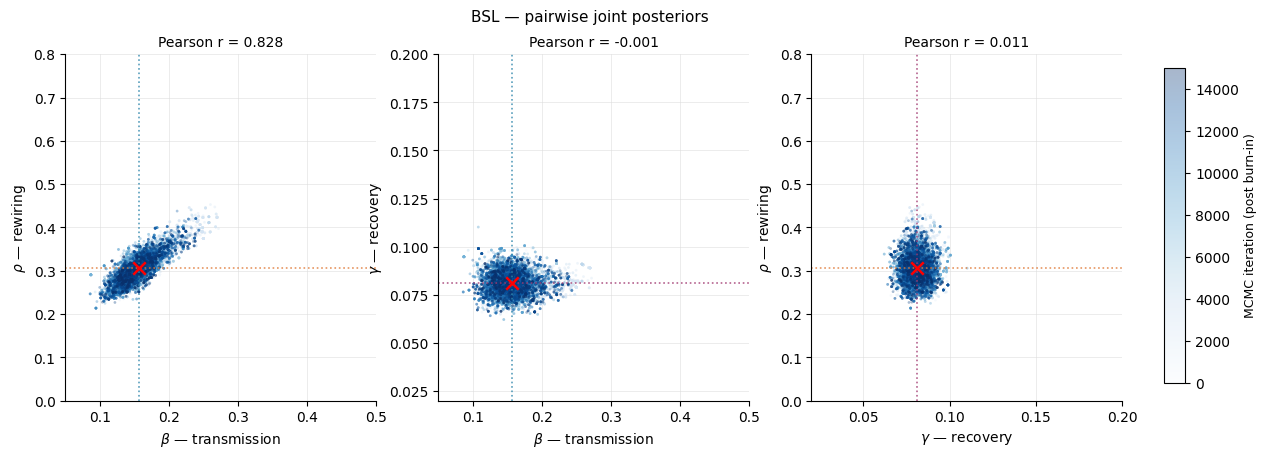
\includegraphics[width=\textwidth]{joint_post_bsl.png}
        \caption{Joint posterior distribution (BSL)}
        \label{fig:joint_post_BSL}
        \centering
    \end{figure}

The weak $\gamma$–$\rho$ correlation ($r \leq 0.05$) is consistent across both methods, confirming that rew\_per\_infected effectively separates recovery from network adaptation. In contrast, the $\beta$–$\rho$ dependence differs markedly: ABC yields a moderate correlation ($r \approx 0.45$), whereas BSL recovers a much stronger association ($r \approx 0.83$). This discrepancy reflects a structural difference between the methods. Rejection ABC compresses the multivariate summary vector into a single Euclidean distance, which can attenuate dependence patterns, while BSL directly models the full covariance structure of the summaries at each proposed $\theta$.

Overall, BSL shows an improvement over ABC, producing more concentrated posteriors and a more coherent dependence structure. Table 6 reports posterior means and 95\% credible intervals under both approaches.

\begin{table}[H]
\centering
\begin{tabular}{lcccc}
\toprule
Parameter & ABC mean & ABC 95\% CI & BSL mean & BSL 95\% CI \\
\midrule
$\beta$  & 0.1770 & $(0.1123,\,0.2578)$ & 0.1567 & $(0.1190,\,0.2011)$ \\
$\gamma$ & 0.0881 & $(0.0613,\,0.1214)$ & 0.0807 & $(0.0703,\,0.0913)$ \\
$\rho$   & 0.3051 & $(0.1940,\,0.4299)$ & 0.3062 & $(0.2563,\,0.3695)$ \\
\bottomrule
\end{tabular}
\caption{Comparison of posterior means and 95\% credible intervals 
         from ABC and BSL.}
\label{tab:ci_comparison}
\end{table}


\section{Conclusion}
This project illustrates both the strengths and limitations of simple
rejection ABC in an adaptive-network epidemic model. While informative
summaries allowed reasonable parameter recovery, the reliance on a scalar
distance and fixed tolerance makes rejection ABC computationally inefficient
and potentially distorts posterior geometry.

Bayesian Synthetic Likelihood addresses some of these issues by replacing
the tolerance with an approximate likelihood, yielding a more concentrated
and structurally coherent posterior. However, further methodological
improvements remain possible.

An implementation of Regression Adjustment \citep{beaumont2002approximate} can be found in the code but is not discussed in this report. Future work could explore SMC-ABC \citep{Sisson2007} and ABC-MCMC \citep{marjoram2013approximation}. Alternatively, Expectation-Propagation ABC \citep{barthelme2014expectation} is of particular interest as it does not require summary statistics and directly approximates the posterior via iterative reverse KL optimisation. However, it has limitations, including a lack of guaranteed convergence and the need for advanced variance reduction methods for stability. 

\section*{Acknowledgement}
\vspace{-1em} % Yes I'm cheating to fit within the 10 page limit
During this project, I came across a \href{https://youtu.be/77yECJ8_dyk?si=wJEvxuK5s3MCoifo}{lecture} by Prof. David Nott on Approximate Bayesian Computation, which provided valuable insight into the topic. While exploring advanced methods, I encountered his work on Bayesian Synthetic Likelihood \citep{Price02012018}. After reaching out to him, he kindly shared additional resources and guidance that helped deepen my understanding. I am sincerely grateful for his time and support.

%
% === BIBLIOGRAPHY =====
%\clearpage
\begingroup
\small
\bibliographystyle{chicago}
\bibliography{references}
\endgroup
	
\end{document}
